\documentclass[10pt]{amsart}

\usepackage{tgpagella}
\fontfamily{qpl}
\usepackage[utf8]{inputenc}
\usepackage{amsmath, amsthm, amscd, amsfonts, amssymb, graphicx, color}
\usepackage[bookmarksnumbered, colorlinks, plainpages=false]{hyperref}
\usepackage{bookmark}
\usepackage{csquotes}
\usepackage{dirtytalk}
\usepackage{float}

\usepackage[dutch]{babel}

\usepackage[style=verbose,backend=biber]{biblatex}
\addbibresource{zotero.bib}
\DeclareBibliographyAlias{artwork}{misc}

\hypersetup{
     colorlinks = true,
     citecolor = blue,
     urlcolor = blue,
     linkcolor = blue,
}

\textheight 22.5truecm \textwidth 14.5truecm
\setlength{\oddsidemargin}{0.35in}\setlength{\evensidemargin}{0.35in}

\setlength{\topmargin}{-.5cm}

\begin{document}
\setcounter{page}{1}

\noindent {\small 2324-S1 werkcollege Oude Geschiedenis}\hfill     {\small \today} \\
% title, issn/data
{\small Opdracht 2: Griekse homoseksualiteit?.}\hfill
{\small } %volume, url

\centerline{}

\centerline{}

\title[Griekse Homoseksualiteit]{Griekse Homoseksualiteit in de klassieke tijd}

\author[J. Vermeltfoort]{Vermeltfoort, Jenny$^1$}

\address{$^{1}$ 3787494, Faculteit Geesteswetenschappen, Leiden
     Universiteit, Leiden, Nederland.}
\email{\textcolor[rgb]{0.00,0.00,0.84}{j.vermeltfoort@umail.leidenuniv.nl}}

%\dedicatory{This paper is dedicated to Professor ABCD}
%\subjclass[2020]{Primary 46L55; Secondary 44B20.}
%\keywords{Analysis, PDEs, algebra, number theory, applied mathematics}
%\date{Received: xxxxxx; Revised: yyyyyy; Accepted: zzzzzz.
%\newline \indent $^{*}$ Corresponding author}

\maketitle

\section*{Opdracht 1}

\noindent In de Spartaanse \textit{age classes} werden homoseksuele relaties aangemoedigd. Dit waren relaties tussen jongens
en ongehuwde jongemannen en waren verbonden aan de oude initiatiepraktijken van de pubers. Deze systematische vorm van
homoseksualiteit kwam enkel in Sparta voor, maar toch werd homoseksualiteit in andere Griekse plaatsen als normaal
bevonden. Binnen de elite van Athene speelde pederastie een belangrijke
rol.\autocite{naereboutOudheidGriekenRomeinen2022}

\section*{Opdracht 2}
\noindent Op de schaal \autocite{dourisAtticRedFigure} staat een oudere man en een jongen afgebeeld. De jongen vertoont nederige
gewoontes, hij kijkt de man niet aan, en draagt zijn kledij over zijn hoofd. De oudere man houd zijn linker hand op
zijn borst en volgens de bron \autocite{dourisAtticRedFigure} heeft hij een kaalgeplukte haan in zijn hand, wat een
liefdes gift representeert. Er van uitgaande dat er werkelijk een liefdes gift word vergeven duid dit op een liefdes
relatie tussen een oudere man en een jongen, wat dus pederastie schetst.

\section*{Opdracht 3}
\noindent In figuur \ref{fig:siana-cup} \autocite{SianaCup575BC} representeert een stuk van een kop, genaamd de \textit{siana
     cup}. Er is een oudere man getoond, links, met een rode baard en een rode borst. Hij heeft zijn linkerhand op de kin
van de jongen, rechts, lang haar, geen baard, en een rode borst. De gewoontes vertonen eigenschappen van een liefdes
relatie en kan daarmee gecategoriseerd worden onder pederastie.
\begin{figure}[H]
     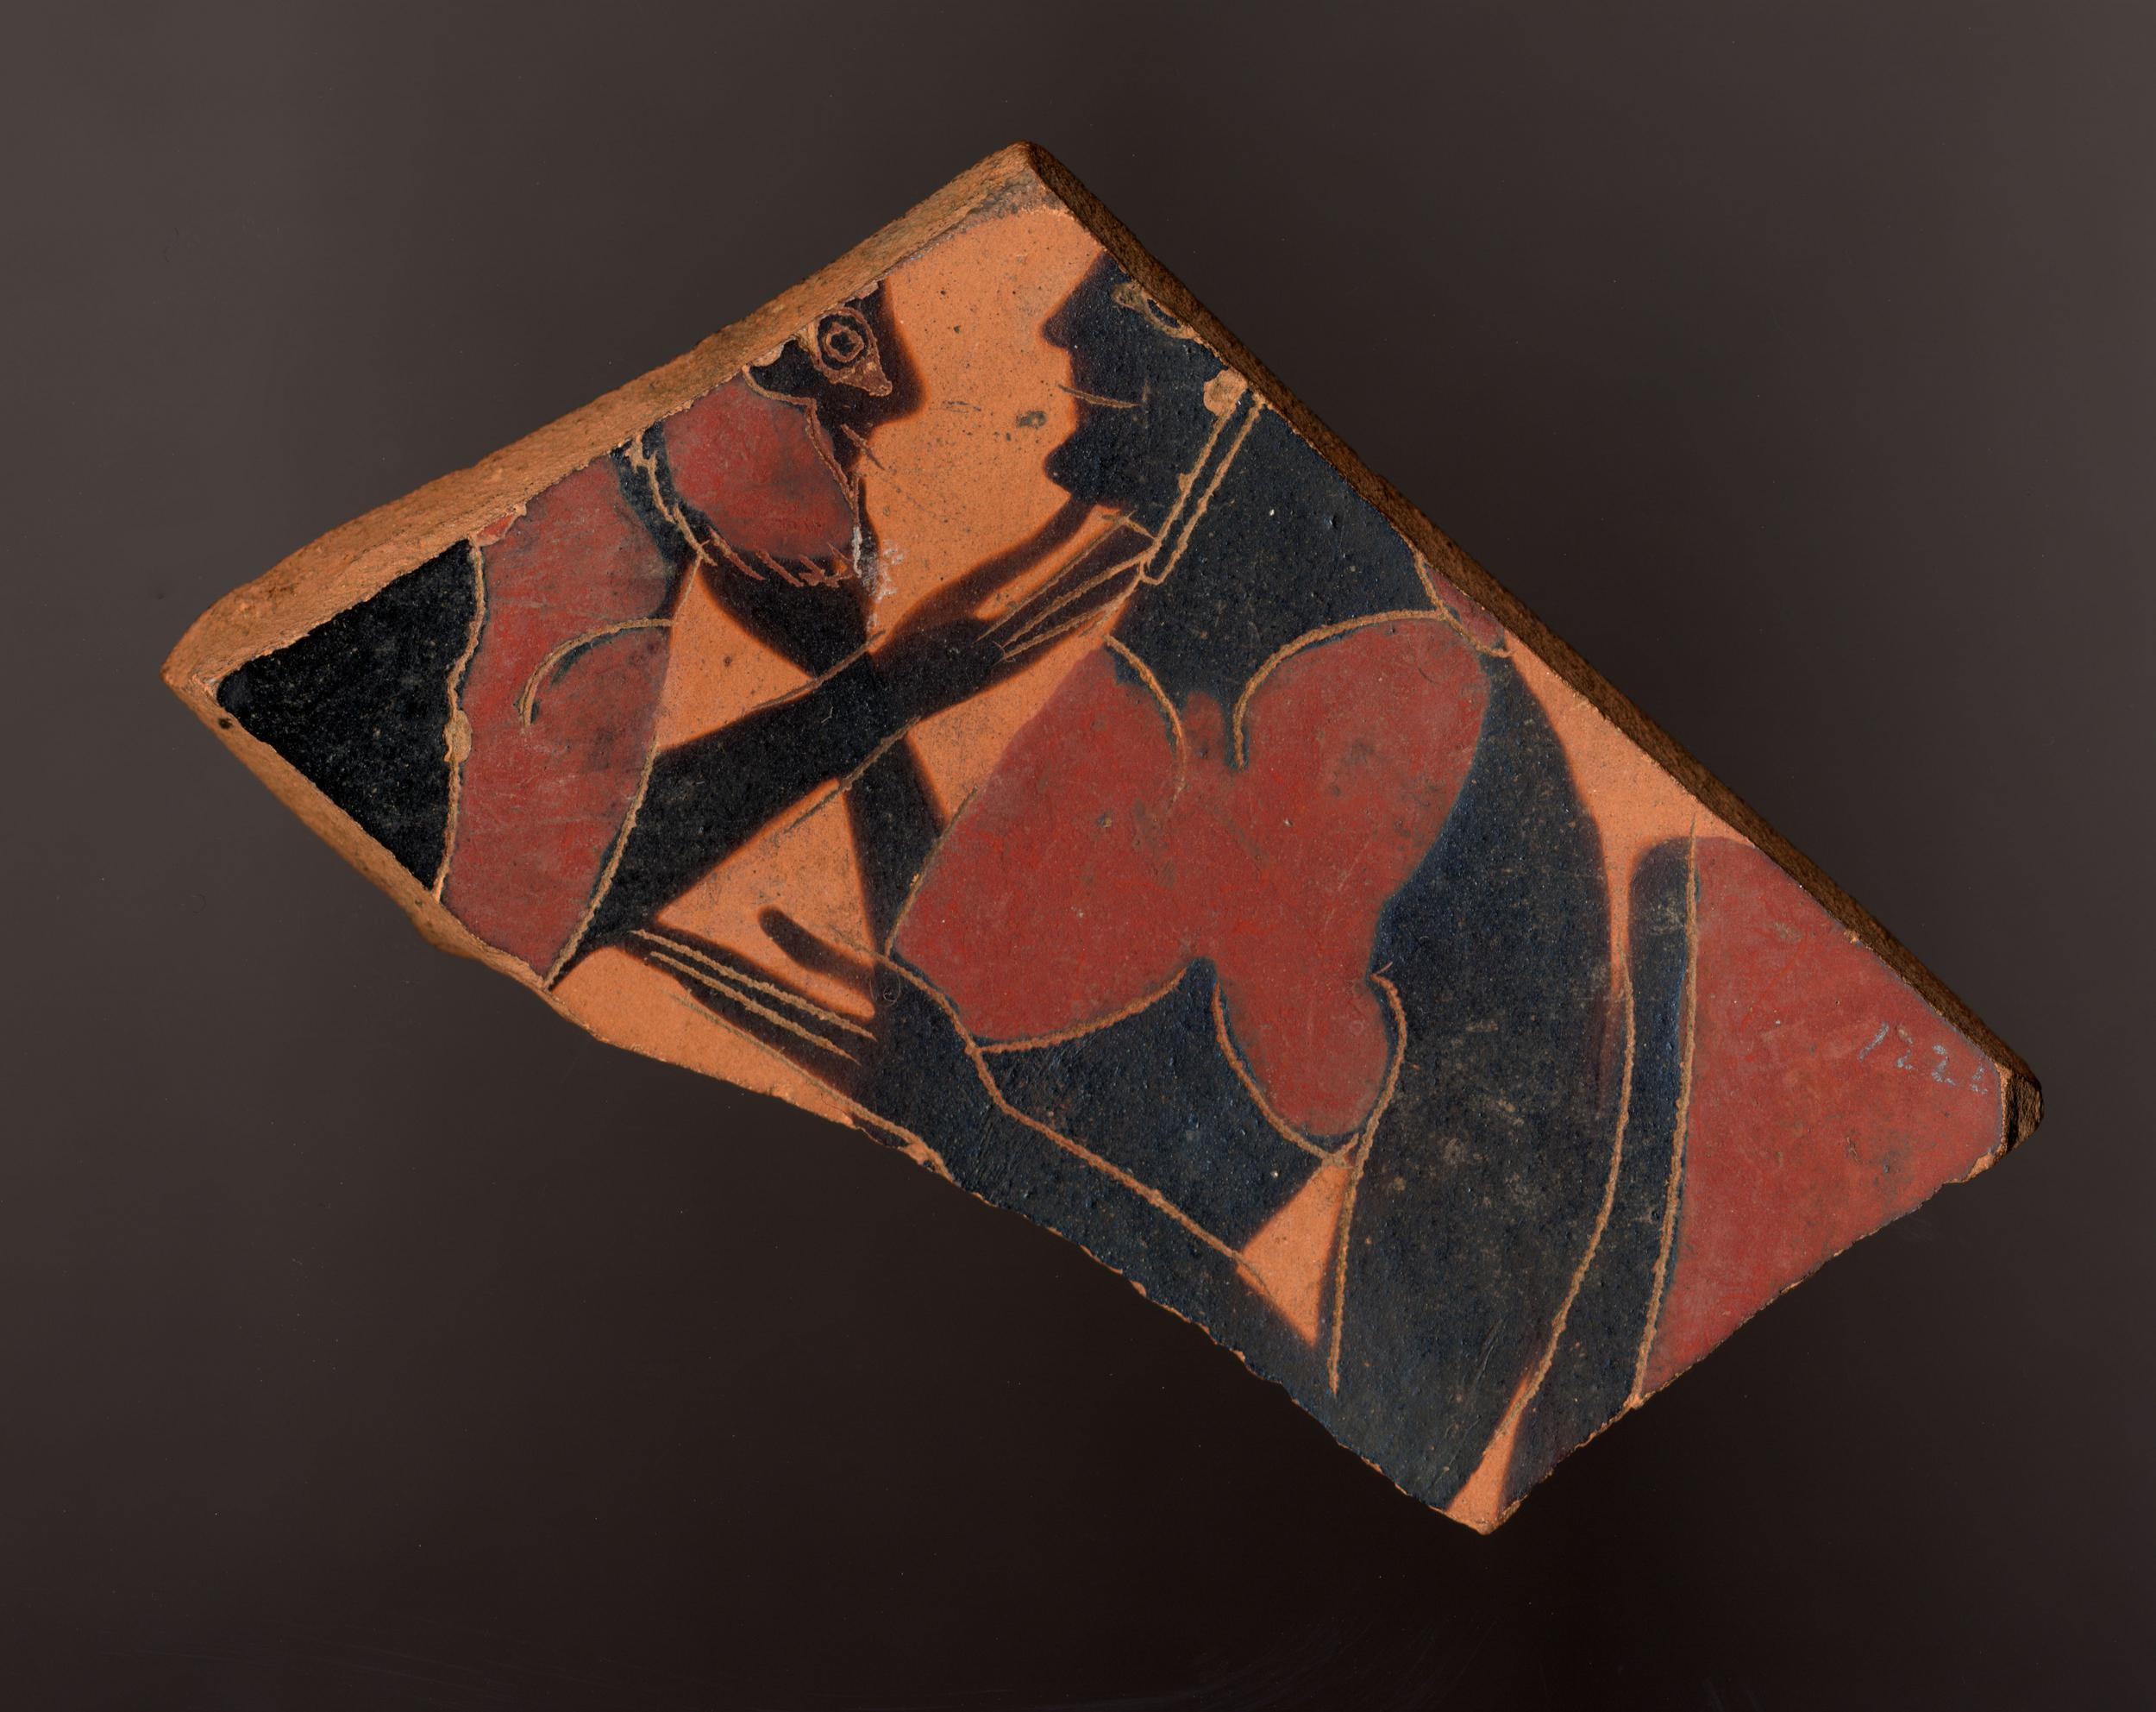
\includegraphics[width=0.5\linewidth]{images/452769001.jpg}
     \caption{Handle of Siana cup: scene of bearded man courting boy.}
     \label{fig:siana-cup}
\end{figure}

\section*{Opdracht 4}
\noindent De tekst van Plutarchus bevestigd dat in Sparta de jongemannen een oog hielden op de jongens. De jongemannen waren
\say{als het ware allemaal de vaders en opvoeders en gouverneurs van alle
     jongens.}\autocite{plutarchusLevenVanPelopidas120} Er word zelfs geconstateerd dat de liefde zorgde voor een sterke
band op het oorlogsveld, omdat \say{minnaars en beminden uit wederzijdse liefde en respect in het gevaar pal stonden
     voor elkaar.}\autocite{plutarchusLevenVanPelopidas120} Dit komt overheen met het beeld wat Naerebout en Singor over
pederastie scheppen, de gelijkenissen komen voort uit de \textit{age classes} maatschappij en het bevestigd dat \say{de
     homoseksualiteit hier misschien verbonden is met de resten van oude initiatiepraktijken die van de pubers mannen
     moesten maken.}\autocite{naereboutOudheidGriekenRomeinen2022}

\section*{Opdracht 5}\label{opdracht5}
\noindent Wat opvallend is aan de bron van Plutarchus \autocite{plutarchusLevenVanPelopidas120} is dat de homoseksualiteit bij de
Spartanen een bepaalde machtsspeling is. De jongens worden gekozen door oudere en status dragende jongemannen. Het is
hiermee niet geheel duidelijk of het hier om werkelijke homoseksualiteit gaat, aangezien de jongens geen andere keuze
hebben. Het hele systeem is ingebakerd in de maatschappij, het is een soort traditie of een standaard proces waar de
leden zich aan vast houden. Hierdoor komen termen zoals acceptatie in deze tijd niet voor, het is voor hun namelijk
vanzelfsprekend.

Merkbaar is dat er voornamelijk geschreven wordt over mannen met status, homoseksualiteit binnen de rest van het volk
word hier uitgesloten. Is dit echter indicatief dat de rest van de bevolking geen homoseksuele relaties ondervond, of
is dit een gevolg van het karakter van de historiografie van deze tijd, waar er enkel geschreven werd over mannen met
aanzien.

\section*{Opdracht 6}\label{opdracht6}
De mens was van oorsprong een gedaante met vier benen, vier armen en twee gezichten. Er waren drie seksen, man-man, vrouw-vrouw en man-vrouw, opeenvolgend representerend, de zon, de aarde en de maan.
Deze gedaantes waren bandeloos en daarom besloot Zeus ze te splitsen. Hieruit ontstond de mens met twee benen. Aangezien de mens nu een helft is van haar gedaante kwam de behoefte om weer geheel te worden op.
Dit is de oorsprong van liefde, waar het gesplitste resultaat van de man-man zocht naar een mannelijke wederhelft, de vrouw-vrouw zocht naar een vrouwelijke wederhelft en de man-vrouw zocht naar een heteroseksueele wederhelft. \autocite{platoSymposium189d-193a}
Wat Aristophanes in \textit{Symposium} beredeneerd is dat de beste mannen voortkomen uit het man-man gedaante, aangezien \say{zij van nature het mannelijkst zijn}\autocite{platoSymposium189d-193a}.

\section*{Opdracht 7}
Wat geconcludeert kan worden uit de tekst van Aristophanes is dat de homoseksuele liefde in Athene geen sociaal construct is zoals dat in Sparta is. De homoseksualiteit wordt gedefinieerd als het verlangen naar een wederhelft van hetzelfde geslacht.
Zijn blik op de man-man kan verklaren hoe er gekeken werd naar de homoseksualiteit van de aristocratie, wat in \hyperref[opdracht5]{Opdracht 5} naar voren komt. Aangezien de beste mannen verlangden naar hun mannelijke wederhelft.

Het is echter belangrijk niet te vergeten dat de tekst van Aristophanes enkel een mythe is en dat het gevaarlijk is om
hieruit informatie uit extrapoleren welke beslaan op de Atheense cultuur en
maatschappij.\autocite{chatgptResponseHoeverreDenk2023}

\section*{Opdracht 8}
Alcibiades is flamboyante aristocraat, Atheense generaal en politicus. Hij was leerling en intieme vriend van Socrates. Mede verantwoordelijk voor de expeditie naar Sicili"e.

\section*{Opdracht 9}
"Attenties door veel mannen met goede afkomst, die klaarblijkelijk diep geraakt waren door zijn stralende jeugdige schoonheid en hem het hof maakten."\autocite{plutarchusLevenVanAlcibiades120}
Dit is hoe Plutarchus de jonge politicus Alcibiades beschrijft.

"Gunsten wedijverden met vleierijen en geschenken", Alcibiades kreeg aanzienlijk veel geschenken, iets wat terug te zin is in \textit{de afbeelding op de drinkschaal}\autocite{dourisAtticRedFigure}.

\section*{Opdracht 10}
Het is moeilijk iets over leeftijdsbeperkingen te halen uit de bron van Aristophanes\autocite{aristophanesKikkers405}. Het toneelstuk werd uitgevoerd een jaar nadat Euripides dood was, hij was 74 jaar oud geworden. Dionysos lijkt een begeerte met zich mee te dragen voor Euripides. Er zou geconcludeerd kunnen worden dat liefde ook de ouderen is toegeschreven.

\section*{Opdracht 11}
Wat Boswell\autocite{boswellChristianitySocialTolerance1980} concludeert dat door verschillende historici
de homoseksualiteit in gemeenschappen van het verleden vaak als onecht worden beschreven. Dus niet conforme
de homoseksualiteit van de moderne gemeenschappen. Er word dus een onderscheid gemaakt tussen het verleden en
nu, dit onderscheid reflecteert de verhouding in leeftijd van de homoseksuele mannen, jongens en mannen.
Hij beweerd echter dat homoseksualiteit in het verleden niet draaide om de leeftijd, knappe mannen werden
als jongen beschreven. Boswell probeert dus te zeggen dat het concept homoseksualiteit in deze tijd kenbaar was en ook zo beschreven werd door Plato; \say{Plato carefully distinguishes in his dialogues between men who are attracted to boys and those who are attracted to other men, but few ancient writers were so careful.}

Halperin\autocite{halperinOneHundredYears1990} heeft bezwaar op deze conclusie, hij gebruikt de bron van Aristophanes
om dit te ontkrachten. Zie \hyperref[opdracht6]{Opdracht 6}, hierop volgend vind Halperin dat Aristophanes niet het
volledige beeld schept. Het lijkt er namelijk op dat Aristophanes niet homoseksualiteit beschrijft zoals wij deze
kennen, zou dit namelijk wel zo zijn dan zou de leeftijdsfactor geen betrekking hebben. Volwassen mannen zouden op
volwassen mannen en jongens op jongens kunnen vallen. Wat Halperin dus concludeert is dat Plato's Aristophanes per
toeval homoseksualiteit schets zoals deze in de moderne wereld wordt gedefinieerd, het doel van de mythe was niet om
homoseksualiteit te beschrijven.

\section*{Opdracht 12}
De noodzakelijke eigenschap van de werkelijke homoseksualiteit kan niet gelinkt worden aan leeftijdsgebonden relaties - zo zouden man en meisje relaties ook als een homoseksuele relatie gezien moeten worden.

Boswell gebruikt de primaire bronnen als voorbeeld van zijn argumenten.

\section*{Opdracht 13}
Aangezien Halperin concludeert dat homoseksualiteit, als begrip, van de moderne tijd en van het verleden verschillen
kan het niet meer zijn dan een sociaal construct.

Halperin gebruikt de mythe van Aristophanes om de argumenten van Boswell to ontkrachten.

\section*{Opdracht 14}
Halperin \autocite{halperinThereHistorySexuality1989} defin"ieerd homoseksualiteit als een een machtsspeling tussen
een persoon van hogere status en zijn onderdaan. Hij verklaard dat homoseksualiteit niet voortkwam uit eigen
verlangens, maar dat dit voortkwam uit culturele gewoontes. Daarmee is homoseksualiteit inherent aan de politieke en sociale sphere van Athene.

\section*{Opdracht 15}
Wat Boswell\autocite{boswellConceptsExperienceSexuality1990} toevoegt aan zijn vorige argument dat er wel degelijk door verschillende
primaire bronnen seksuele voorkeuren voortkomen uit aantrekkingskracht naar een bepaald geslacht. Dit behelpt zijn argument tegen Halperin,
aangezien Halperin beargumenteerde in zijn werk dat deze seksuele voorkeur ontbrak binnen Plato's Aristophanos.

\section*{Opdracht 16}
Persoonlijk concludeer ik dat beide argumenten relevant zijn. De definitie van homoseksualiteit zoals deze in de moderne wereld wordt beschreven is niet dezelfde vorm als de homoseksualiteit van het verleden. De sociale
en culturele context is hier van relevantie.
Zoals het woordenboek van Dale\autocite{Homoseksueel2023} homoseksualiteit beschrijf als \say{met seksuele gevoelens voor leden van het eigen geslacht.} Hier ligt de nadruk op seksuele \textbf{gevoelens}, wat niet direct te verhalen is uit de primaire bronnen van Aristophanes\autocite{aristophanesKikkers405} en Plato\autocite{platoSymposium189d-193a}. De manier waarop deze primaire bronnen \say{homoseksualiteit} beschrijven lijkt inderdaad meer op een sociaal construct zoals Halperin\autocite{halperinThereHistorySexuality1989} dat beschrijft. Liefde is namelijk een vrij algemeen begrip en representeert daarmee niet direct de gevoelens zoals deze in de moderne wereld worden bevonden. Homoseksualiteit in deze tijd zou pas dermate gelijk getrokken kunnen worden met de moderne term wanneer er een persoonlijke bron naar voren treed, een bron waar het verlangen, de obsessie, de belangeloze acties richting een geliefd persoon van hetzelfde geslacht worden beschreven. De huidige bronnen spreken enkel over homoseksualiteit vanuit een buitenstaand perspectief en daarmee is het verhaal niet compleet.

\section*{Opdracht 17}
Abductieve beredenering is een methode waarbij een mogelijke verklaring wordt gegeven op een observatie. Een voorbeeld hiervan is:
\begin{enumerate}
     \item Mijn computer muis doet het niet.
     \item Een computer muis doet het niet met een lege batterij.
     \item De batterij van mijn muis is leeg.
\end{enumerate}
Waar redenering 3 een voorbeeld is van abductieve beredenering, aangezien er ook andere redenen kunnen zijn waarom mijn muis het niet doet. Om meer eigenschappen te defini"eren is het noodzakelijke om een uitgebreidere observatie te bevestigen, echter is dit voor abductieve beredenering niet noodzakelijk. Er wordt enkel een mogelijke verklaring gegeven voor een verschijnsel.

Het gebruik van de bron \textit{Symposium} \autocite{platoSymposium189d-193a} door Boswell en Halperin kan als een
voorbeeld beschouwd worden van abductieve beredenering. De autheurs gaan in op een bron welke een mythe beschrijft,
daarmee mist het volledige beeld van homoseksualiteit. Er worden aannames gemaakt, wat ertoe leid dat de gegeven
conclusie een beschrijving \textbf{kan} zijn van homoseksualiteit in het verleden.

\section*{Opdracht 18}

Queer theorie is het analyseren van het verleden met als middel de identiteitskarakteristieken van moderne tijd. In het
verleden waren termen zoals lgbtq+, ras, nationaliteit, klasse, en burgerschap niet deel van het gemeenschappelijke
bewust zijn. Concreet waren deze vormen van deze definities wel aanwezig, maar de mens uit het verleden had niet de
kunde om dit te beschrijven of om zich hier aan te koppelen. Hiervoor zijn sociale en culturele raamwerken
noodzakelijk, zonder de juiste structuren binnen de maatschappij kan er niet gedacht worden aan termen welke de norm
verbreken.

Zo zijn er bepaalde aspecten aan de moderne tijd waardoor het bewust zijn van dit soort sociale meta informatie vorm
krijgen. Door de huidige informatie cultuur zijn uitzonderlijke ervaringen niet langer uniek, ervaringen worden
interactief gedeeld met een hele wereld, hierdoor is het makkelijker voor minderheden samenhang te vinden. Dit
verschild met het verleden, waar sociale interacties groot en deels beperkt waren tot de kleine gemeenschappen waar de
mens woonde. Door de wetenschap kunnen bepaalde ervaringen, gevoelens, en menselijke verschillen een plaats krijgen
binnen een identiteit. Wetenschap maakt deze verschillen concreet door onderzoek, waardoor het gegrond word binnen de
realiteit.

\newpage \printbibliography{}

\end{document}

%------------------------------------------------------------------------------
% End of journal.tex
%------------------------------------------------------------------------------
